\chapter{Impacte ambiental} \label{impacte}
% Veure altres projectes: https://upcommons.upc.edu/pfc/?locale=es

\section{Impacte de l'estudi d'Experiència d'Usuari}
El projecte consisteix en un estudi sobre una aplicació per a \gls{smartphone}. El temps invertit en el desenvolupament d'aquest estudi es pot classificar en:

\begin{description}
\item[PFC] Inclou l'anàlisi, disseny i prototipatge (exceptuant els prototips programats), redacció de la memòria, entrevistes amb el tutor etc.
\item[Cursos] Són cursos sobre \gls{Android} i Java que s'han efectuat per poder aprendre a crear aplicacions per aquest sistema.
\item[Programació Android] Inclou el temps invertit programant els diversos prototips i parts d'aquests que han estat programats.
\end{description}


\begin{table}
\centering
\begin{tabular}{ | l | r | r |}
\hline
\headB{Part} & \headB{Temps invertit [h]} & \headB{Consum elèctric [kWh]} \\
\hline
PFC & 281 & 28,08\\
\hline
Cursos & 130 & 13,25\\
\hline
Programació & 471 & 48,00\\
\hline
\end{tabular}
\caption{Hores invertides en l'estudi i consum que representa}
\label{table:impact}
\end{table}

A la taula \ref{table:impact} i a la figura \ref{fig:impact} es poden veure les hores invertides en l'estudi. Durant tot l'estudi s'ha fet servir un ordinador amb una potència mitjana de 100W. A més a més, per a la programació i pels cursos s'ha fet servir un \gls{Nexus_5}, amb una potència mitjana de 2W. 


\begin{figure}[ht]
\centering
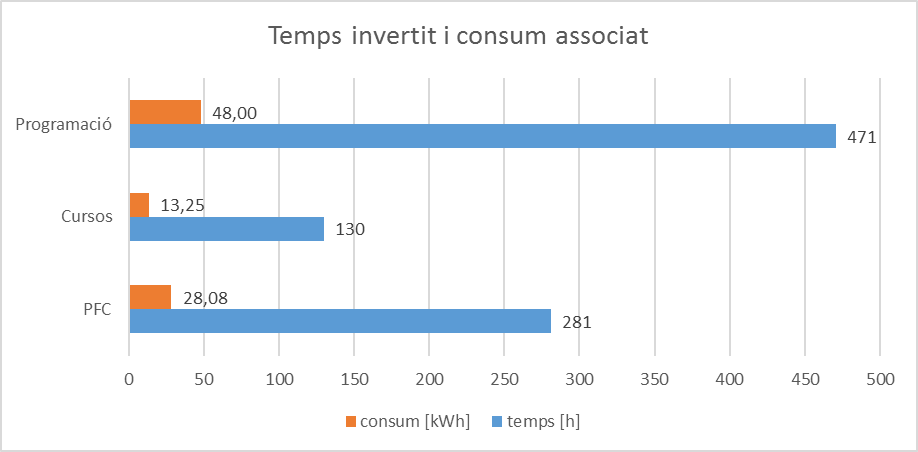
\includegraphics[scale=0.6]{Impact.png}
\caption{Temps invertit i consum associat}\label{fig:impact}
\end{figure}

A part del consum energètic, també cal considerar el consum de paper. Tot i que s'ha intentat reduir al mínim el seu ús, en algunes parts de l'estudi era necessari, concretament s'ha emprat:

\begin{description}
\item[Plantilles per al disseny:] 22 
\item[Plantilles per a l'avaluació:] 25
\item[Varis:] 5
\end{description}

És a dir, en total s'ha emprat 52 fulls de paper.

\section{Impacte de l'ús de l'aplicació}
Tot i que en aquest projecte només s'ha arribat a crear un prototip, aquest ha estat dissenyat per a que en un futur es pugui posar al mercat una aplicació per a la gestió de despeses domèstiques. Com a tal, s'espera que en un futur modifiqui els hàbits d'alguns usuaris a l'hora de gestionar la seva economia personal, ajudant per una banda a prescindir de l'ús de paper. També s'espera que alguns usuaris canviïn l'ús d'ordinadors per al de \glspl{smartphone} amb el conseqüent estalvi energètic. Això però és més difícil de quantificar ja que depèn de la quantitat d'usuaris que acabin fent servir l'aplicació a més a més del sistema de gestió que utilitzaven prèviament. 
